\documentclass[a4paper,12pt]{article}
\usepackage{indentfirst}
\usepackage[utf8x]{inputenc}
\usepackage[T1]{fontenc}
\usepackage[hmargin={30mm,15mm},vmargin={20mm,20mm},bindingoffset=0mm]{geometry}
\usepackage[onehalfspacing]{setspace}
\usepackage[colorlinks=true, linkcolor=blue, citecolor=blue, urlcolor=blue, unicode]{hyperref}
\usepackage{amsmath}
\parindent=7mm
\usepackage{graphicx}
\renewcommand{\refname}{Literatūros sąrašas} % article
%\renewcommand{\bibname}{Literatūros sąrašas} % report
\renewcommand{\contentsname}{Turinys}
\renewcommand{\figurename}{Iliustracija}

\begin{document}
\thispagestyle{empty} % nerasomas psl. nr

\begin{center}
 VILNIAUS UNIVERSITETAS 
 
MATEMATIKOS IR INFORMATIKOS FAKULTETAS

MATEMATINĖS INFORMATIKOS KATEDRA

\vspace{4cm}

\textbf{Motiejus Ėringis}

Informatikos studijų programa

Matematinės informatikos šaka


\vspace{3cm}

\textbf{\Large Kompiuterinė rega. Transporto priemonių valstybinių numerių aptikimas.}

Tiriamojo seminaro ataskaita

\vspace{4cm}

\vfill

Vilnius \ \  2015
\end{center}

\clearpage

%\maketitle 

\newpage
\tableofcontents

\newpage

\section*{Įvadas}
\addcontentsline{toc}{section}{Įvadas} % rasoma turinyje

Kompiuterinė rega – tai mokslo šaka, tirianti metodus, kaip iš vaizdų išgauti mus dominančią informaciją bei kaip tuos vaizdus apdoroti. OpenCV – tai viena pupliariausių kompiuterinės regos apsimokančių algorimų bibliotekų. Išleista 2000 metais ir ligšiol tobulinama. OpenCV populiarumą nulėmė tai, kad ji yra:
\begin{itemize}
  \item Atviro kodo
  \item Nemokama
  \item Turi programavimo sąsajas C++, C, Python, Java, MATLAB/OCTAVE kalboms.
\end{itemize}

Mano tikslas šiame seminare buvo susipažinti su OpenCV bibliotekos teikiamomis galimybės ir pabandyti įgyvendinti nesudėtingą programą, gebančią filmuotoje medžiagoje aptikti tranporto priemonių valstybinius numerius ir pagal jų atstumo pokyti nustatyti greičio reikšmę.


\newpage

\section{Bendras programos veikimo algoritmas}
Iliustracijoje ~\ref{fig:BendrasAlgoritmas} pateikiamas apibendrintas seminare sukurtos programos algoritmas. Šioje programoje buvo pasinaudota pavyzdiniu kodu pateikiamu drauge su knyga „Mastering OpenCV with Practical Computer Vision Projects“ \cite{MasteringOpenCV}.

\begin{figure}[h!]
  \caption{Bendras programos veikimo principas.}
  \centering
    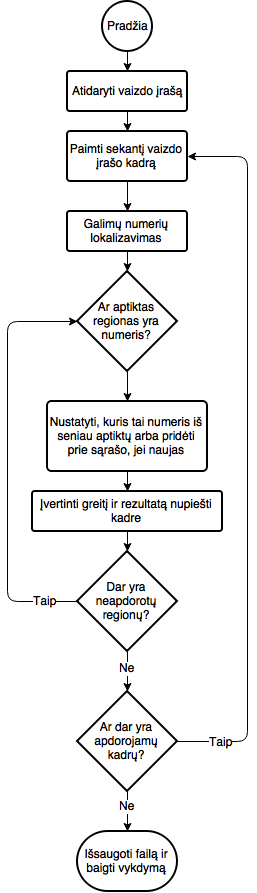
\includegraphics[width=0.3\textwidth]{algo1.png}
  \label{fig:BendrasAlgoritmas}
\end{figure}

\subsection{Numerių aptikimas}

\subsubsection{Suskirtymas regionais}
Analizuoti kadrą pradedame pritaikydami greyscale filtrą ir dar keletą kitų. Tada išskiriame regionus su findContours funkcija. Iš aptiktų regionų sąrašo tolesnei analizei mes pasiliekame tik tuos regionus, kurių kraštinių santykis yra artimas 520/110 = 4,727272 (numerių santykis, kaip matosi iliustracijoje ~\ref{fig:Numeriai}). Tada regionas dar yra patikslinamas su 10 atsitiktinių taškų, iš kurių floodFill algoritmas besiplėsdamas randa pakankamai tikslias numerio ribas.

\begin{figure}[h!]
  \caption{Ispaniškų valstybinių numerių dimensijos. Mus dominančios dimensijos nesiskiria nuo lietuviškų valstybinių numerių.}
  \centering
    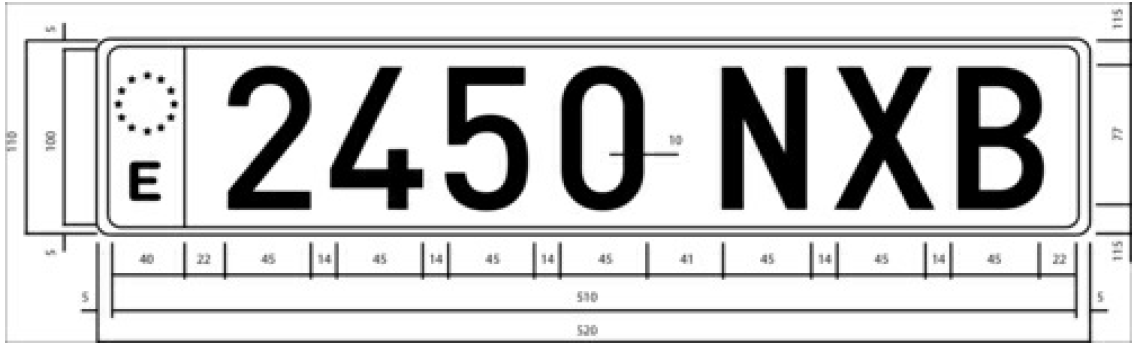
\includegraphics[width=1\textwidth]{numeriai.png}
  \label{fig:Numeriai}
\end{figure}

\subsubsection{SVM klasifikavimas}
Kai turime apdorotus kadro segmentus, kurie potencialiai galėtų būti numeriai, mum reikia nuspręsti, ar konkretus segmentas yra numeris ar nėra. Šiam tikslui naudojamas atraminių vektorių klasifikatoriaus (Support Vector Machine – SVM) algoritmas. SVM yra struktūros atpažinimo algoritmas sukurtas dvejetainei klasifikacijai. Šis algoritmas save apsimoko iš mūsų pateiktų duomenų. Turime algoritmui pateikti mokymosi medžiagą – fotografijas su numeriais ir be jų tam, kad algoritmas sukurtų hiperplokštumas, pagal kurias galėtų klasifikuoti duomenis.


\subsection{Greičio įvertinimas}
Greičiui nustatyti reikalingi du dalykai – atstumas ir laikas. Laiką nesunkiai gauname iš video failo kadrų dažnio, o atstumą galime nustatyti pagal numerių pločio taškų skaičių ir naudojamos vaizdo kameros židinio nuotolį.


\subsubsection{Greičio formulė}
\begin{equation}
\overline{greitis} = \frac{\Delta atstumas}{\Delta laikas}
\end{equation}


\subsubsection{Atstumo nustatymas}
\begin{figure}[h!]
  \caption{Jei žinomas vaizdo kameros židinio nuotolis ir daikto aukštis, tai pagal panašių trikampių savybę galime nustatyti atstumą nuo vaizdo kameros iki daikto.}
  \centering
    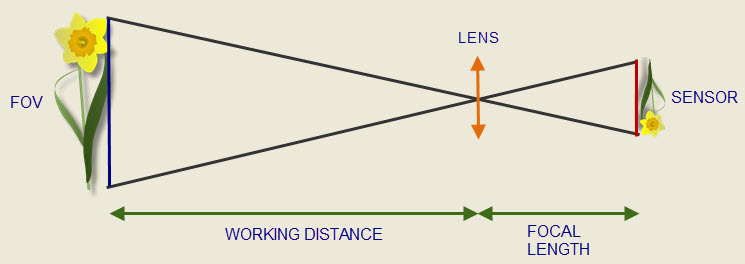
\includegraphics[width=0.8\textwidth]{lens.jpg}
  \label{fig:Lens}
\end{figure}

Žinomas numerių plotis D. Padarome nuotrauką su žinomu atstumu iki numerių Z. Išmatuojame numerių plotį gautais taškais - d. 
Židinio nuotolis:
\begin{equation}
 f =\frac{d Z}{D}
\end{equation}
Pagal panašių trikampių sąvybę galime apskaičiuoti dabartinį atstumą Z' iki kameros:
\begin{equation}
Z'= \frac{D' f}{d}
\end{equation}


\subsubsection{Tų pačių numerių nustatymas}
Kadangi vaizdo įrašas yra apdorojamas kadras po kadro, norint nustatyti, kad numeris yra tas pats numeris ir šitame kadre, mums reikia konteksto iš senesnių kadrų. Kiekvieną sykį, kai SVM nustato, jog regionas yra numeris, jis yra įtraukiamas į numerių sąrašą ir nustatoma nulinė išsekimo laiko žymeklio reikšmė. Jei toks numeris jau yra sąraše (laikome, kad numeris yra tas pats, jei stačiakampiai susikerta), tai tik jo laiko žymeklis yra nustatomas į nulį. Apdorojant naują kadrą visų numerių išsekimo laiko žymeklis yra padidinamas. Jei išsekimo laiko žymeklis viršija nustatytą reikšmę, tai numeris yra šalinamas iš sąrašo. Kadangi ne kiekviename kadre sėkmingai aptinkami tie patys numeriai, ši logika leidžia mums nepamesti numerio, jei keliolika kadrų būtų neatpažinta.


\section*{Rezultatas}
\addcontentsline{toc}{section}{Rezultatas} % rasoma turinyje
Seminaro metu sėkmingai pavyko parašyti programą, kuri geba aptikti ir nustatyti transporto priemonių greitį pagal numerius. Iliustracijoje ~\ref{fig:Kadras} greitis išvedamas taškais per sekundę, nes tuo metu duomenys apie židinio nuotolį nebuvo turimi.
\begin{figure}[h!]
  \caption{Kadro dalis iš vaizdo įrašo apdoroto seminaro metu sukurta programa. ID - aptikimo numeris, o V - greitis. Čia židinio nuotolio duomenimis nesinaudojama.}
  \centering
    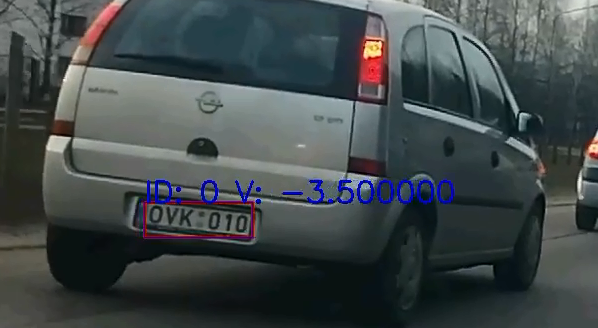
\includegraphics[width=0.8\textwidth]{kadras.png}
  \label{fig:Kadras}
\end{figure}

\section*{Išvados}
\addcontentsline{toc}{section}{Išvados} % rasoma turinyje
Seminaro metu susipažinta su OpenCV bibliotekos teikiamomis galimybėmis. Nors rezultatas tikrai nėra komercinio lygio, tačiau įdėjus daugiau darbo tokia programinė įranga potencialiai galėtų būti naudojama kelių policijos veikloje.
 
\newpage
 
\begin{thebibliography}{99}
\addcontentsline{toc}{section}{Literatūra} %% Literatura bus itraukta i turini
\bibitem {wikicv}
\url{https://en.wikipedia.org/wiki/Computer_vision} 

\bibitem {wikiopencv}
\url{https://en.wikipedia.org/wiki/OpenCV} 

\bibitem {MasteringOpenCV}
 
Daniel Lélis Baggio, Shervin Emami, David Millán Escrivá, Khvedchenia Ievgen, Naureen Mahmood, Jason Saragih, Roy Shilkrot \textit{Mastering OpenCV with Practical Computer Vision Projects}, Packt Publishing, 2012, p. 148-171

\bibitem {Regitra}
\url{http://www.regitra.lt/lt/transporto_priemoniu_registravimas/valstybinio_numerio_zenklai}

\bibitem {svmLT}
\url{http://www.mif.vu.lt/~bastys/academic/ATE/biometrika/SVM.pdf}

\end{thebibliography} 
 
\end{document}
